\documentclass[12pt]{article}

\usepackage[utf8]{inputenc}
\usepackage[russian]{babel}
\usepackage{geometry}
\usepackage{graphicx}
\usepackage{soul}
\usepackage{color}
\usepackage{colortbl}

\geometry{a4paper, top=15mm, bottom=15mm, left=10mm, right=10mm}

\begin{document}

\setcounter{page}{0}
\thispagestyle{empty}

\begin{center}
    Федеральное государственное автономное учебное учреждение высшего образования\\
    <<Национальный исследовательский университет ИТМО>>\\
\vspace{0.5cm}
    Мегафакультет компьютеных технологий и управления\\
    Факультет программной инженерии и компьютерной техники
\end{center}

\vspace{3cm}

\begin{center}
\Large
\textbf{
    Отчёт\\
    по лабораторной работе №3\\
    по дисциплине <<Программирование>>
}
\end{center}

\begin{center}
\large
    Вариант 31180120
\end{center}

\vspace{6cm}

\begin{flushright}
    Студент: Кожухин Иван Алексеевич, группа P3118\\
    Преподаватель: Письмак Алексей Евгеньевич
\end{flushright}

\vspace{6cm}

\begin{center}
    Санкт-Петербург\\
    2022
\end{center}

\newpage

\tableofcontents

\newpage

\section{Задание}

По заданной предметной области построить объектную модель. Программа должна удовлетворять следующим требованиям:\\
\\
1. Доработанная модель должна соответствовать принципам SOLID.\\
2. Программа должна содержать как минимум два интерфейса и один абстрактный класс (номенклатура должна быть согласована с преподавателем).\\
3. В разработанных классах должны быть переопределены методы equals(), toString() и hashCode().\\
4. Программа должна содержать как минимум один перечисляемый тип (enum).\\
\\
Порядок выполнения работы:\\
\
1. Доработать объектную модель приложения.\\
2. Перерисовать диаграмму классов в соответствии с внесёнными в модель изменениями.\\
3. Согласовать с преподавателем изменения, внесённые в модель.\\
4. Модифицировать программу в соответствии с внесёнными в модель изменениями.\\
\\
Текст задания варианта:\\
\\
\textit{Кроме заботы о пище, Жулио проявил также заботу о чистоте. Поскольку топить лишний раз печь им было лень, а по ночам бывало зябко, Жулио придумал спать не на кроватях, а в сундуках. Забравшись вместе с периной в сундук и закрывшись в нем крышкой, можно было согреть дыханием воздух и спать, не ощущая холода.}

\newpage

\section{Ход работы}

Исходники кода программ и файлов:\\
\\
\textbf{https://github.com/troublegale/ProgLab3}

\begin{figure}[h]
    \centering
    
\includegraphics{image1.png}
    \caption{QR-код для доступа к репозиторию на GitHub}
\end{figure}

\begin{figure}[h]
    \centering
    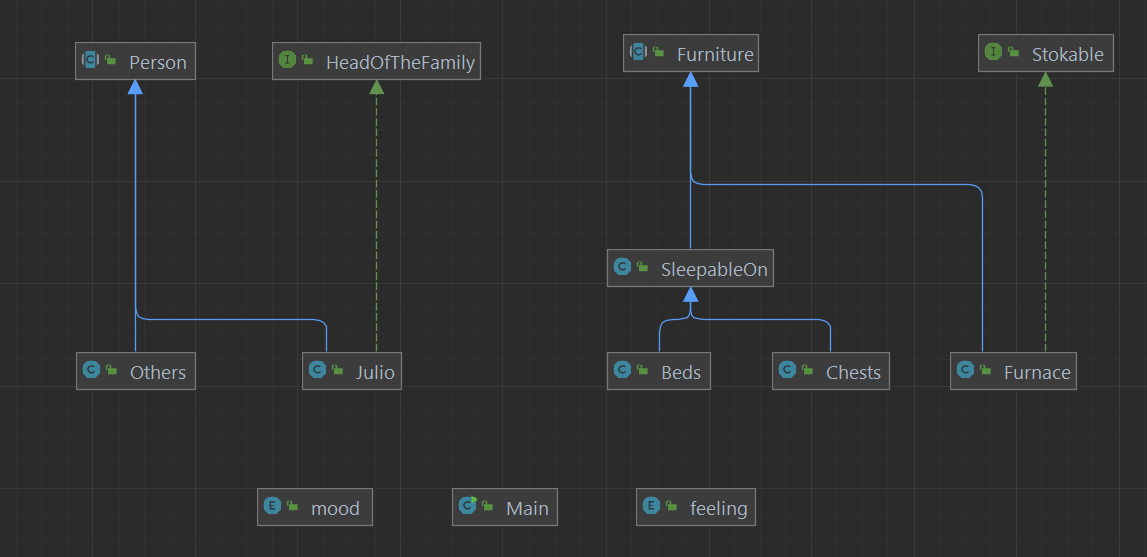
\includegraphics[width=\linewidth]{image2.png}
    \caption{Диаграмма классов объектной модели}
\end{figure}

\begin{figure}[h]
    \centering
    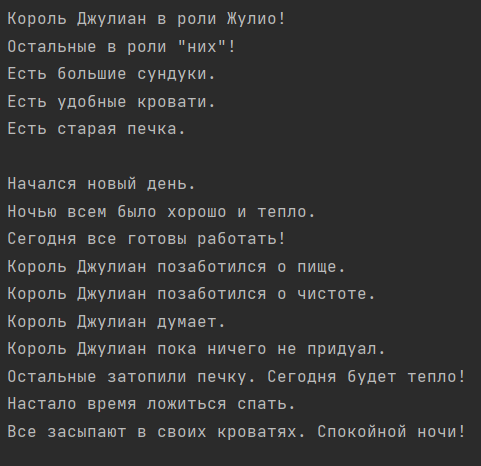
\includegraphics[width=0.6\linewidth]{image3.png}
    \caption{Пример вывода программы, часть 1}
\end{figure}
\newpage
\begin{figure}[h]
    \centering
    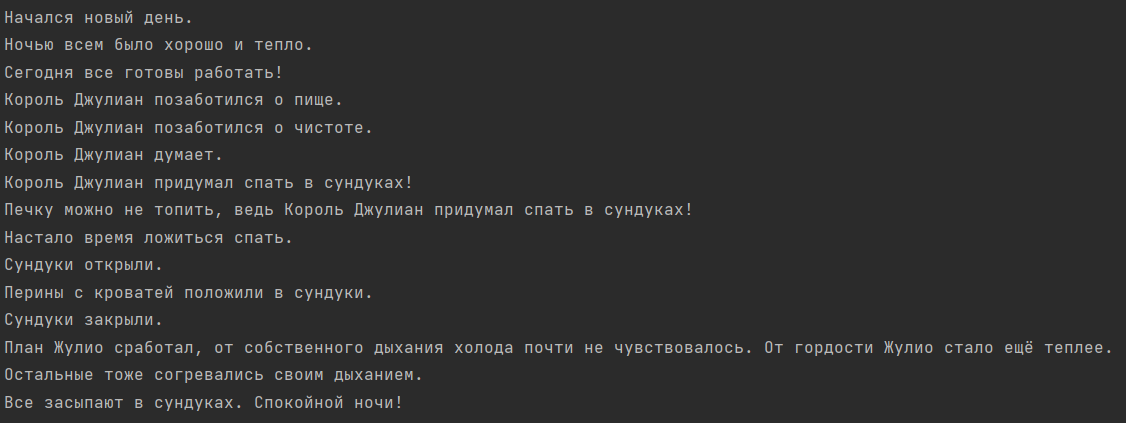
\includegraphics[width=\linewidth]{image4.png}
    \caption{Пример вывода программы, часть 2}
\end{figure}

\newpage

\section{Вывод}

В ходе лабораторной работы я ознакомился с принципом SOLID, научился строить объектную модель по краткому описанию предметной области, а также углубил свои знания о принципах и понятиях ООП на языке Java.

\end{document}